We ran the random switch state explorer 1000 times on the previously
introduced Swiss suburban grid (\autoref{fig:data_prep:swiss_suburb_topology_patched}).
The values obtained for all operational
measures (\autoref{sec:operational_measures}) as well as the switch state scores
(\autoref{sec:score}) can be seen as histograms in \autoref{fig:result:suburban:histograms}.

\begin{figure}[H]
  \begin{subfigure}{.33\textwidth}
    \centering
    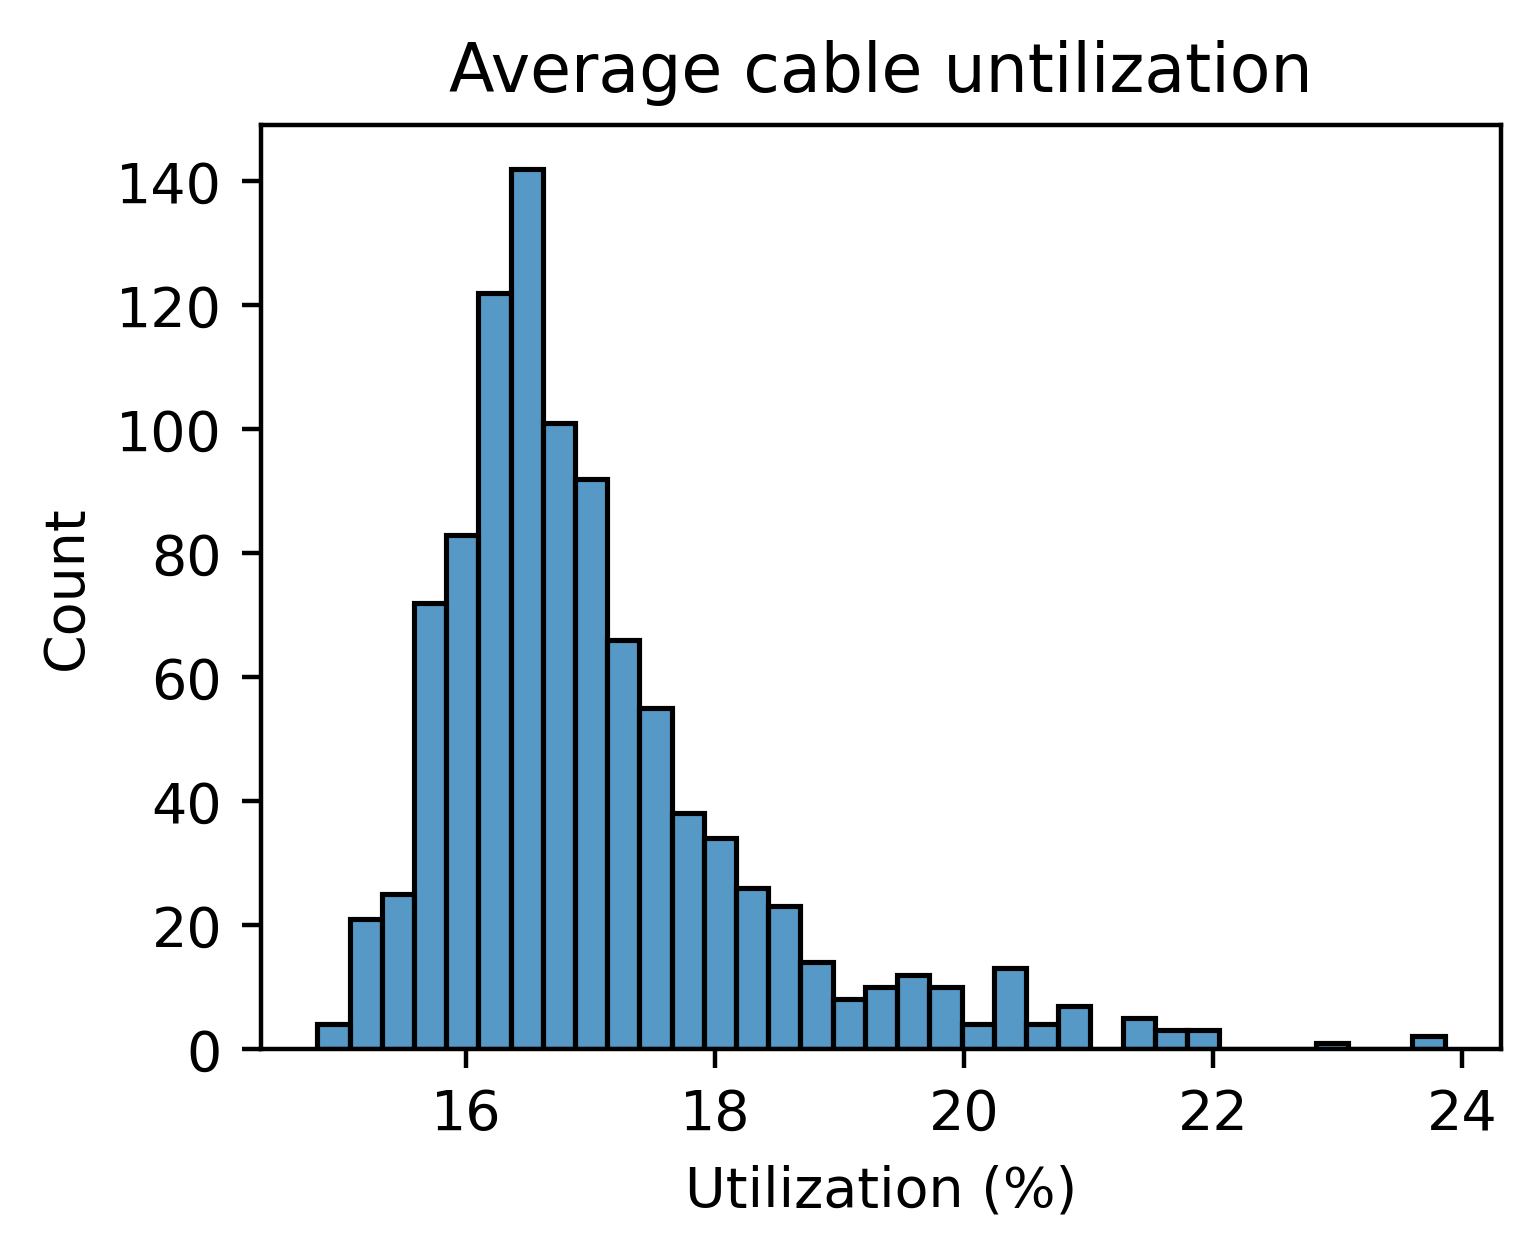
\includegraphics[width=\linewidth]{img/switchstate_exploring/swiss_suburb/histograms/avg_cable_util.png}
    \caption{}
    \label{fig:result:suburban:histograms:avg_cable}
  \end{subfigure}%
  \begin{subfigure}{.33\textwidth}
    \centering
    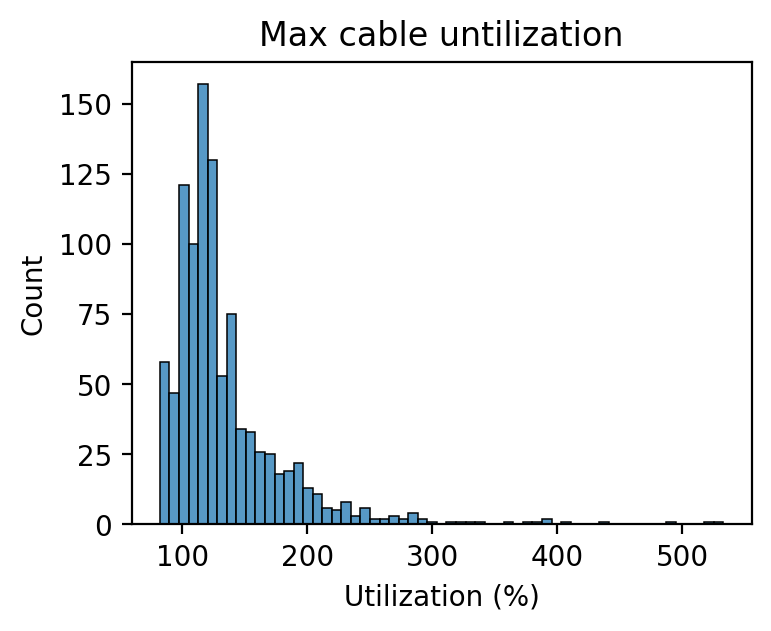
\includegraphics[width=\linewidth]{img/switchstate_exploring/swiss_suburb/histograms/max_cable_util.png}
    \caption{}
    \label{fig:result:suburban:histograms:max_cable}
  \end{subfigure}
  \begin{subfigure}{.33\textwidth}
      \centering
      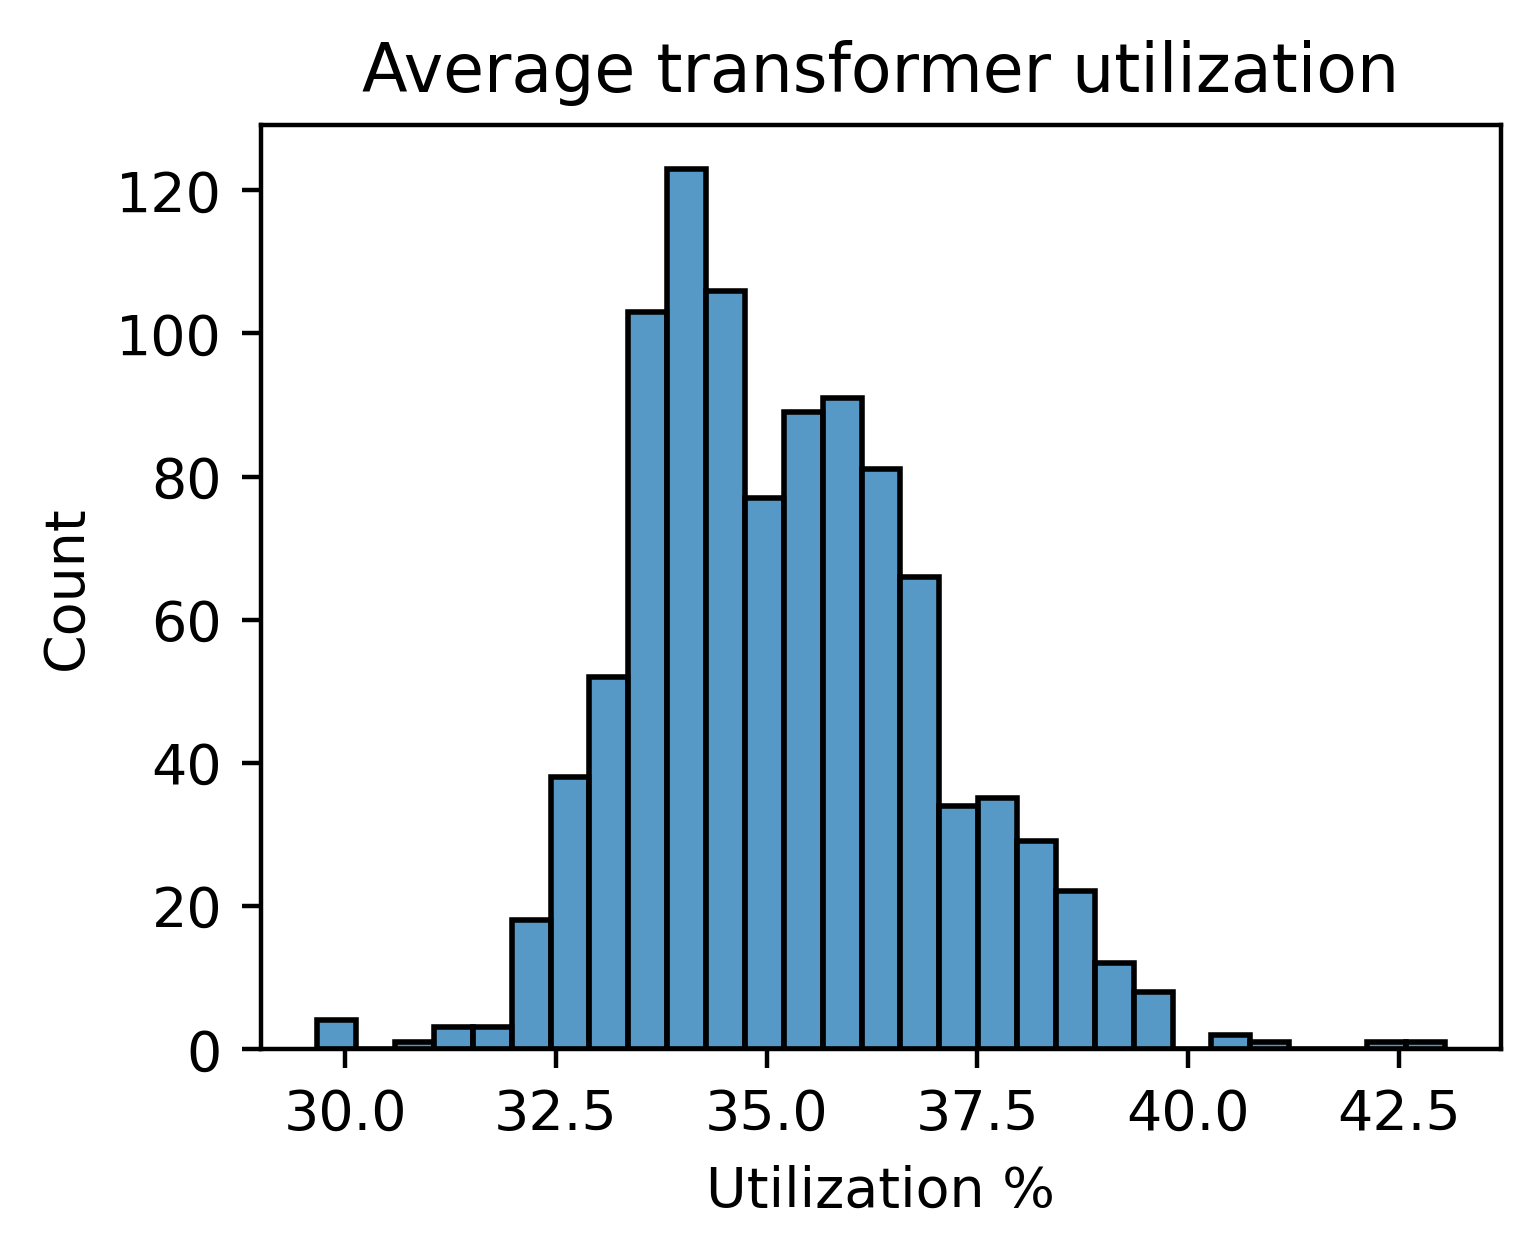
\includegraphics[width=\linewidth]{img/switchstate_exploring/swiss_suburb/histograms/avg_trafo_util.png}
      \caption{}
      \label{fig:result:suburban:histograms:avg_trafo}
    \end{subfigure}\\
    \begin{subfigure}{.33\textwidth}
      \centering
      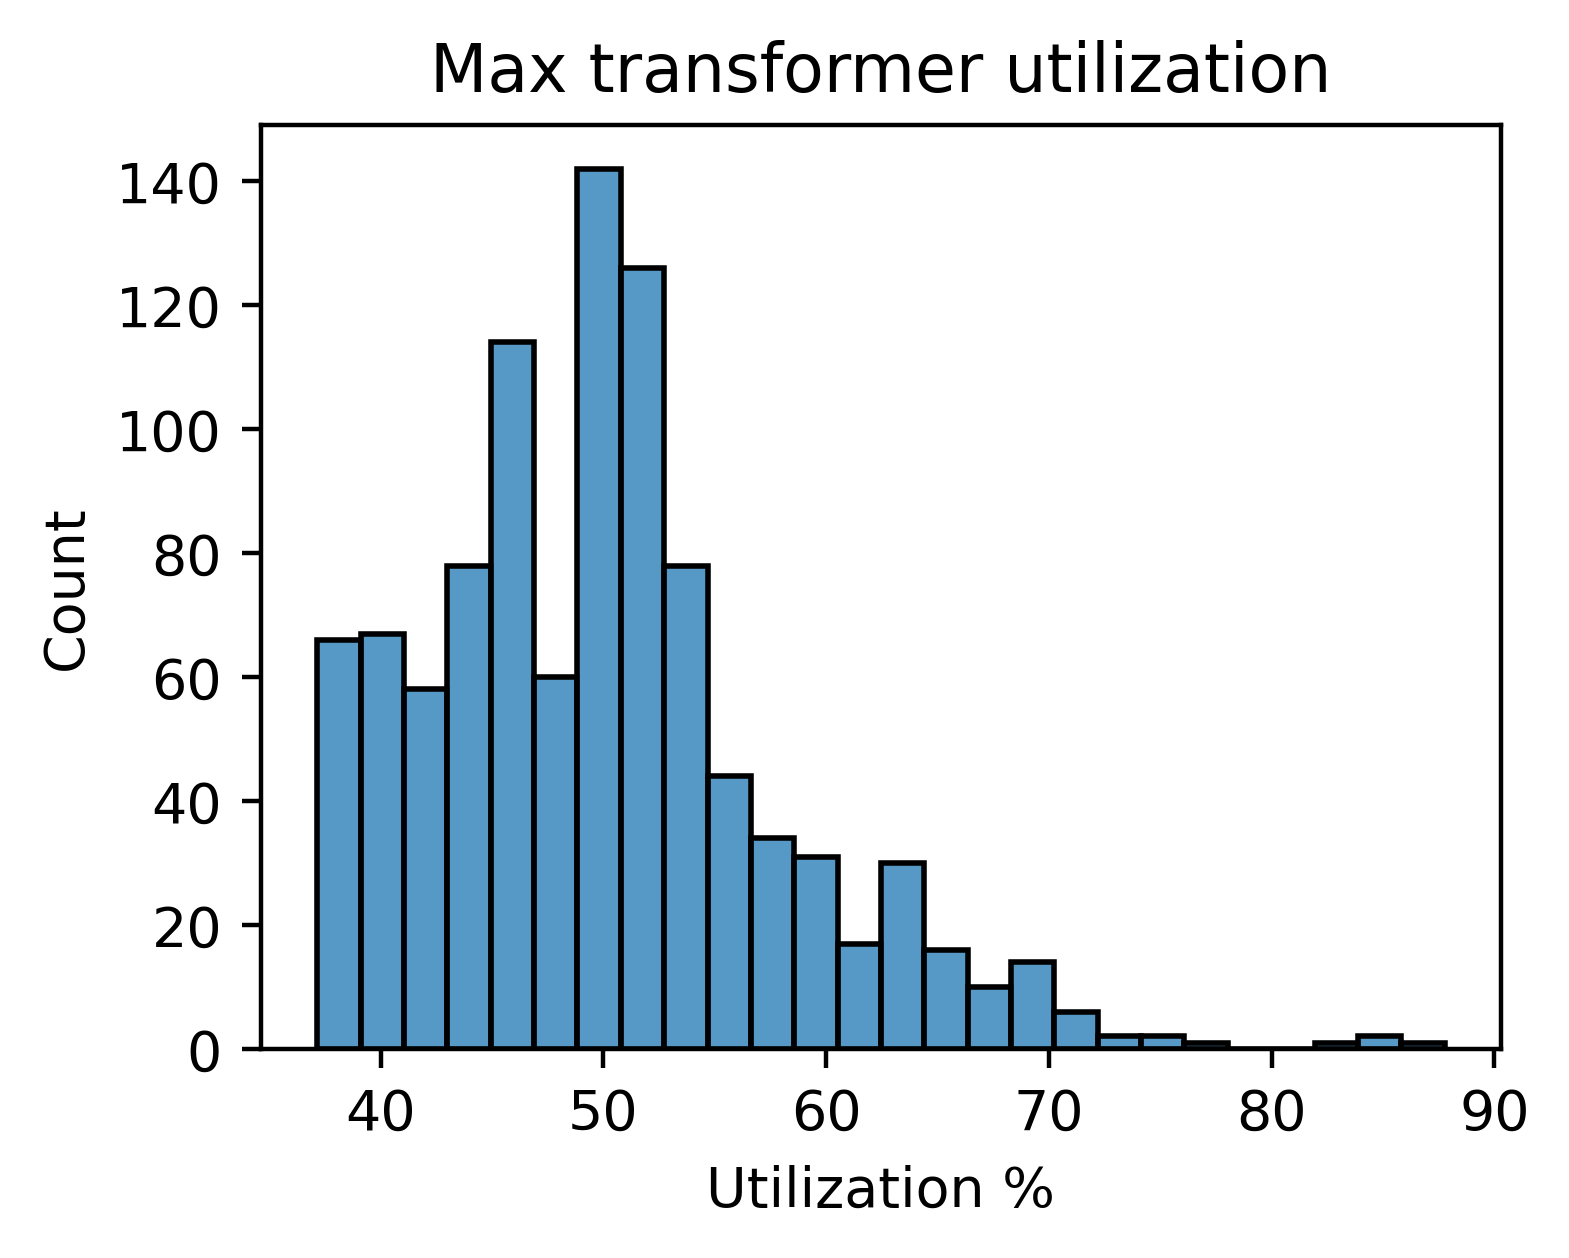
\includegraphics[width=\linewidth]{img/switchstate_exploring/swiss_suburb/histograms/max_trafo_util.png}
      \caption{}
      \label{fig:result:suburban:histograms:max_trafo}
    \end{subfigure}%
    \begin{subfigure}{.33\textwidth}
      \centering
      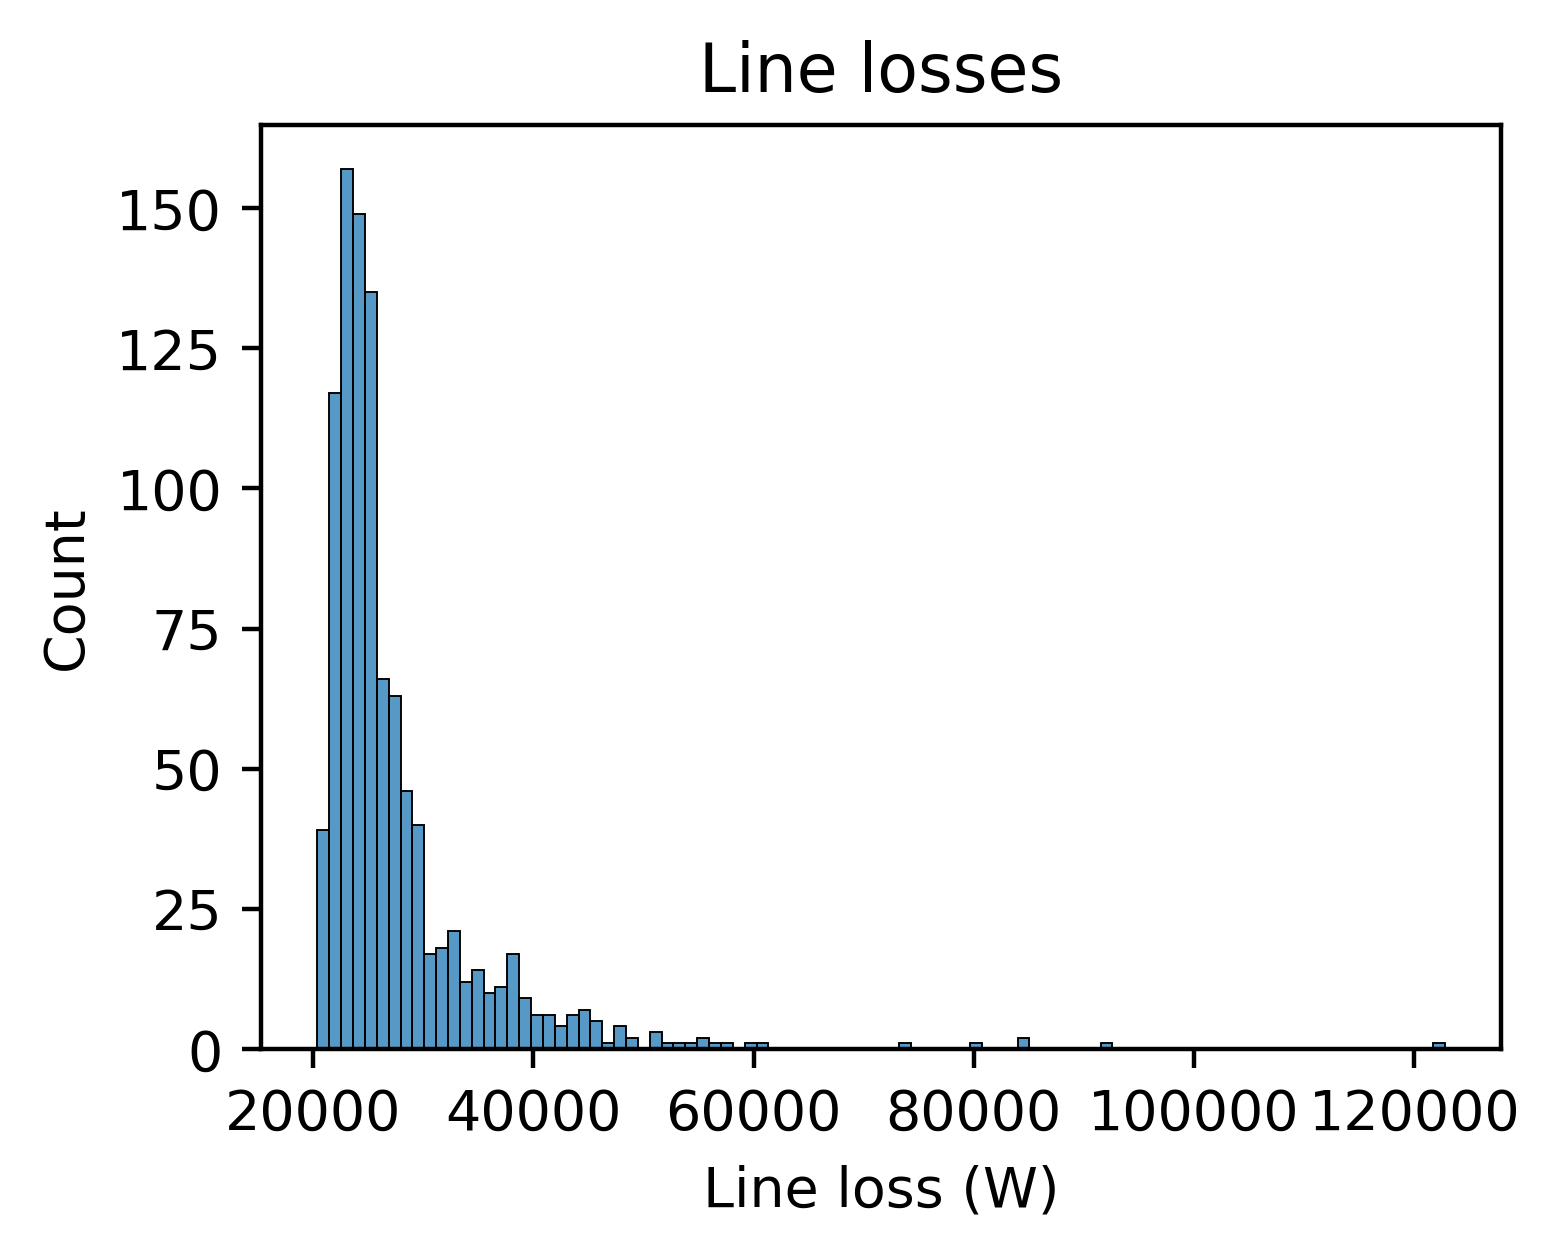
\includegraphics[width=\linewidth]{img/switchstate_exploring/swiss_suburb/histograms/line_loss.png}
      \caption{}
      \label{fig:result:suburban:histograms:line_loss}
    \end{subfigure}%
    \begin{subfigure}{.33\textwidth}
      \centering
      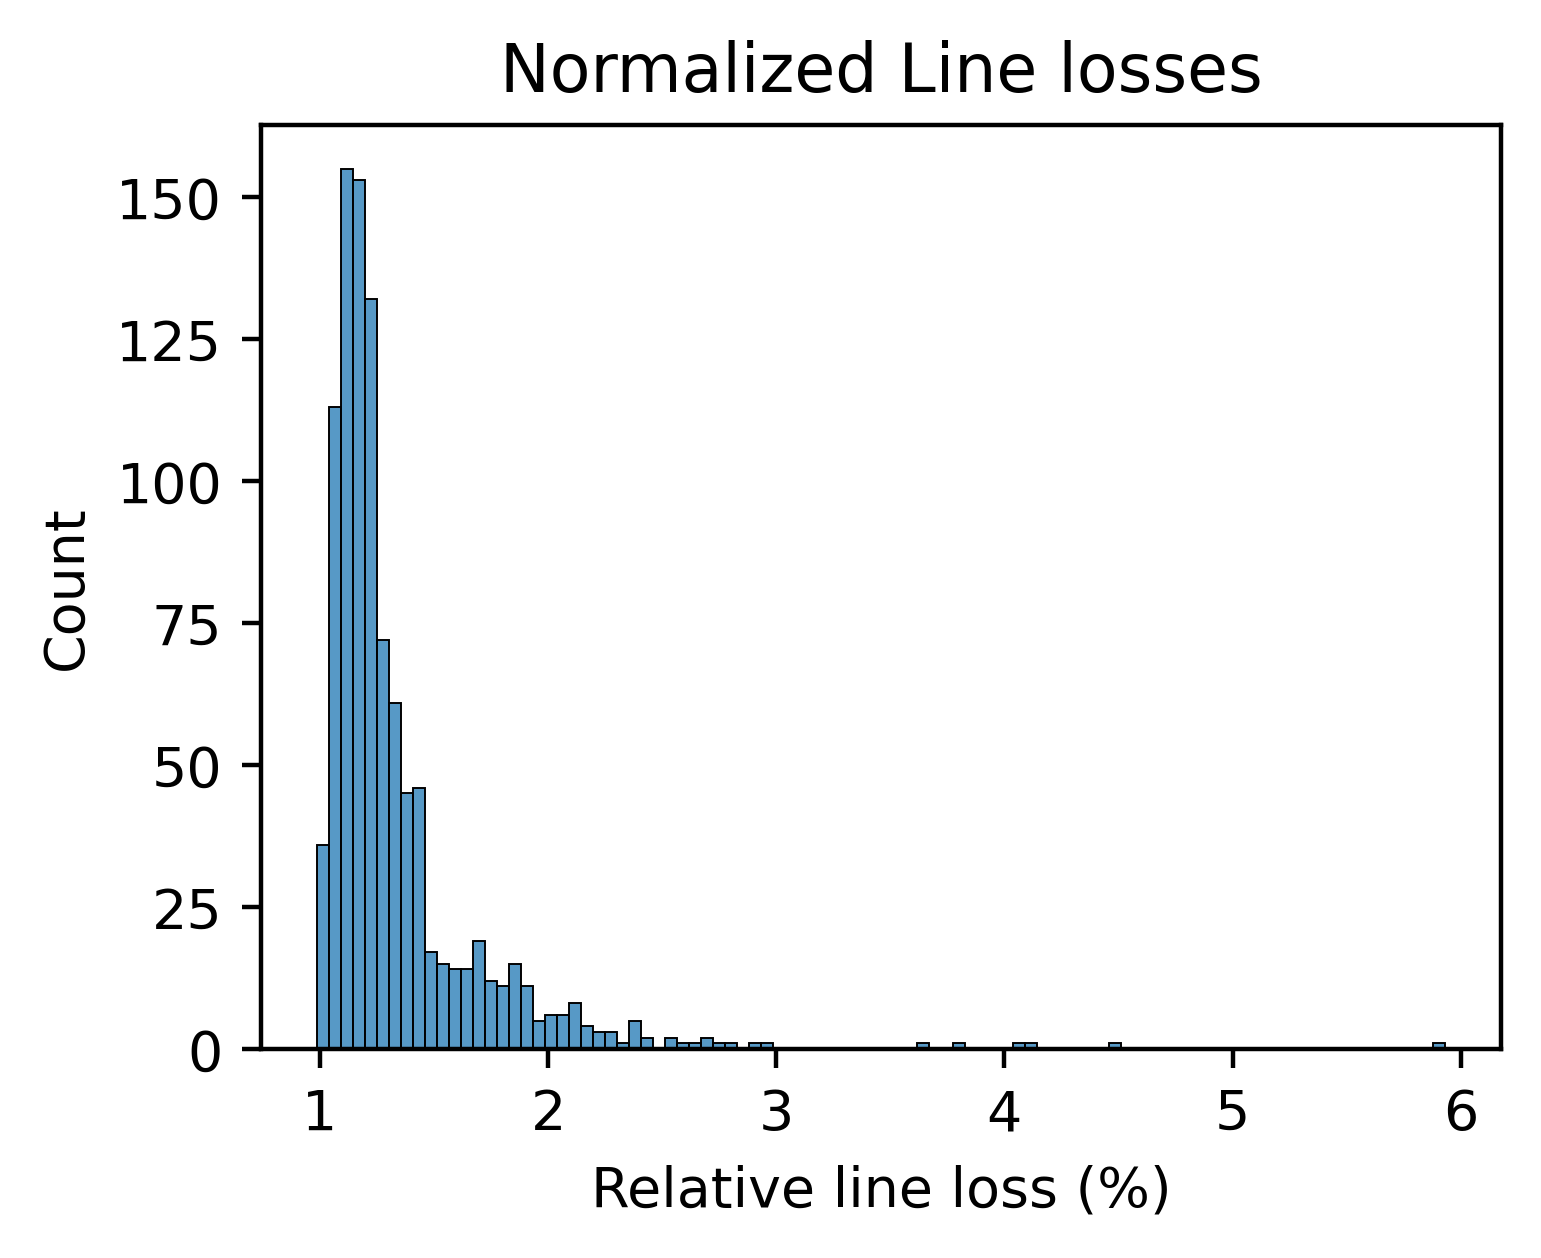
\includegraphics[width=\linewidth]{img/switchstate_exploring/swiss_suburb/histograms/line_loss_relative.png}
      \caption{}
      \label{fig:result:suburban:histograms:line_loss_rel}
    \end{subfigure}\\
    \begin{subfigure}{.33\textwidth}
      \centering
      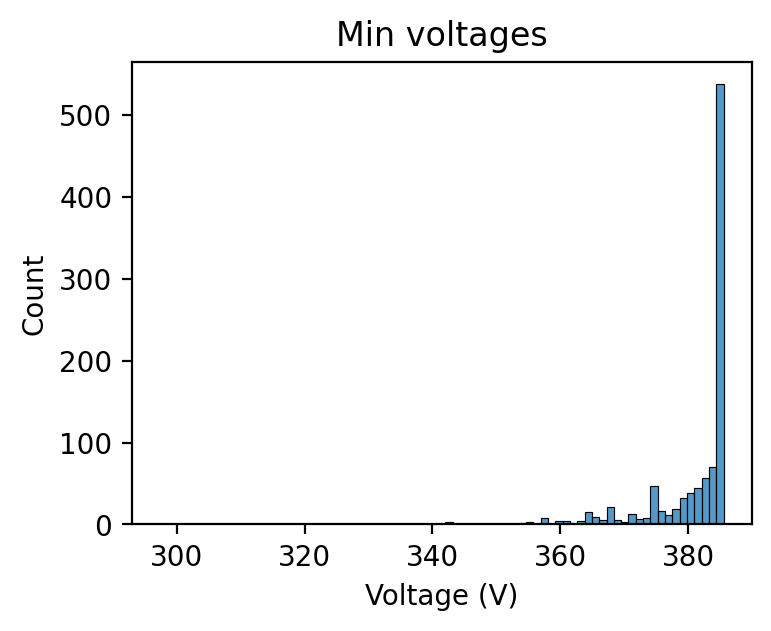
\includegraphics[width=\linewidth]{img/switchstate_exploring/swiss_suburb/histograms/min_voltage.png}
      \caption{}
      \label{fig:result:suburban:histograms:min_voltage}
    \end{subfigure}%
    \begin{subfigure}{.33\textwidth}
      \centering
      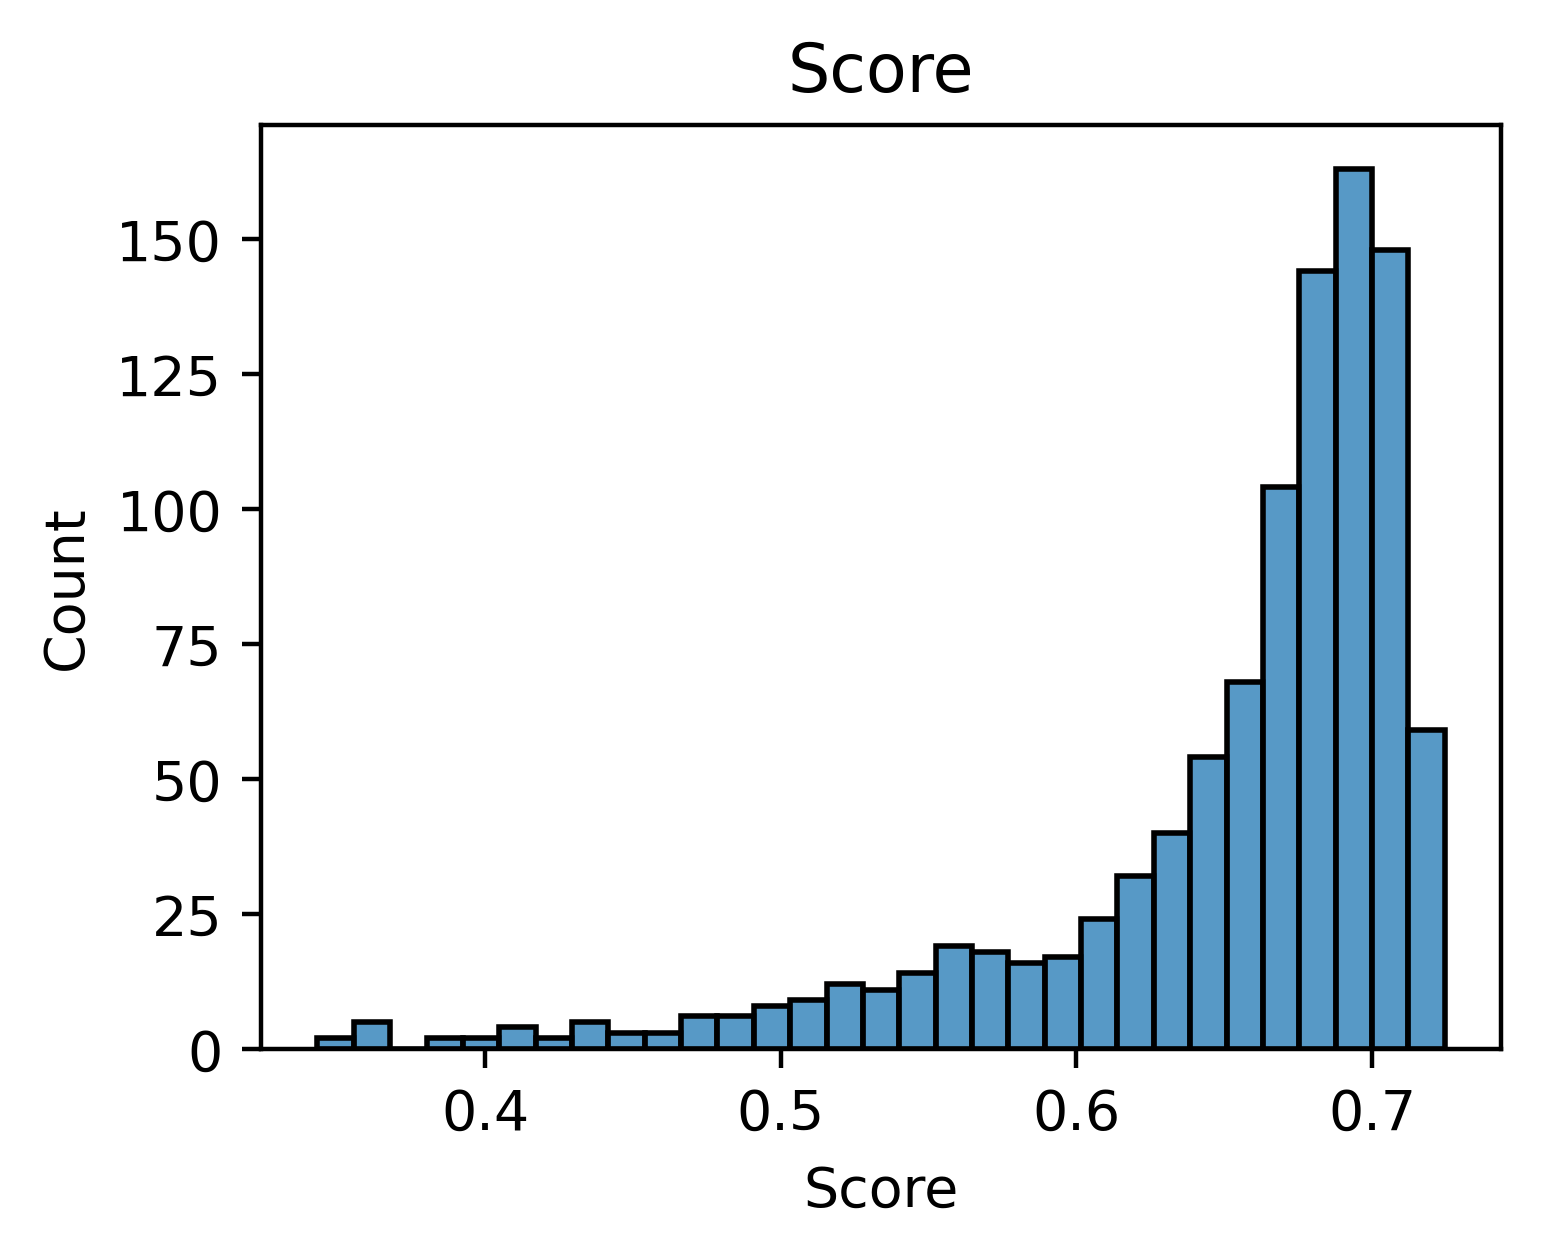
\includegraphics[width=\linewidth]{img/switchstate_exploring/swiss_suburb/histograms/score.png}
      \caption{}
      \label{fig:result:suburban:histograms:score}
    \end{subfigure}
  \caption{Power produced/consumed by a household (a) and a solar panel (b) within a SimBench grid at different times of day and at different times of year. Data is generated by a standard laod profile model within VEP and obtained over API\autocite{venios}}
  \label{fig:result:suburban:histograms}
\end{figure}

The most surprising result from these was that good switch states are not rare. Table
\ref{fig:result:suburban:table} shows a comparison between the best switch state found
and the SSS. There it can be seen that the SSS only reaches a score of $62.5$.
Looking this value up in \autoref{fig:result:suburban:histograms:score} shows,
that most switch states generated are better than the SSS. In the case
of this grid area the biggest improvements can be observed for the max cable
utilization (\autoref{eq:measures:cable_utilization}) and max transformer
utilization (\autoref{eq:measures:trafo_utilization}) with smaller improvements
in other categories. This is a very promising result when it comes to future
grid expansion. The main restriction on if new prosumers can be connected are
the utilization values of cables and transformer. Thus, these results suggest
that many additional prosumers could be connected to the grid
"for free" simply through switching action.


\begin{figure}[H]
  \centering
  \begin{tabular}{lrr}
    \toprule
    & SSS & Best random switch state \\
    \midrule
    Score (x100) & 62.5 & 72.5 \\
    Min. Voltage (V) & 381.2 & 385.5 \\
    Max. cable utilization (\%) & 167.0 & 87.0 \\
    Avg. cable utilization (\%) & 16.1 & 16.4 \\
    Max. transformer utilization (\%) & 69.0 & 39.6 \\
    Avg. transformer utilization (\%) & 38.4 & 32.5 \\
    Toal line losses (kW) & 44.1 & 37.1 \\
    \bottomrule
  \end{tabular}
  \caption{
    Grid performance of SSS and best random switch case obtained
    through 1000 samples
  }
  \label{fig:result:suburban:table}
\end{figure}
  

\begin{figure}[H]
  \begin{subfigure}{.5\textwidth}
      \centering
      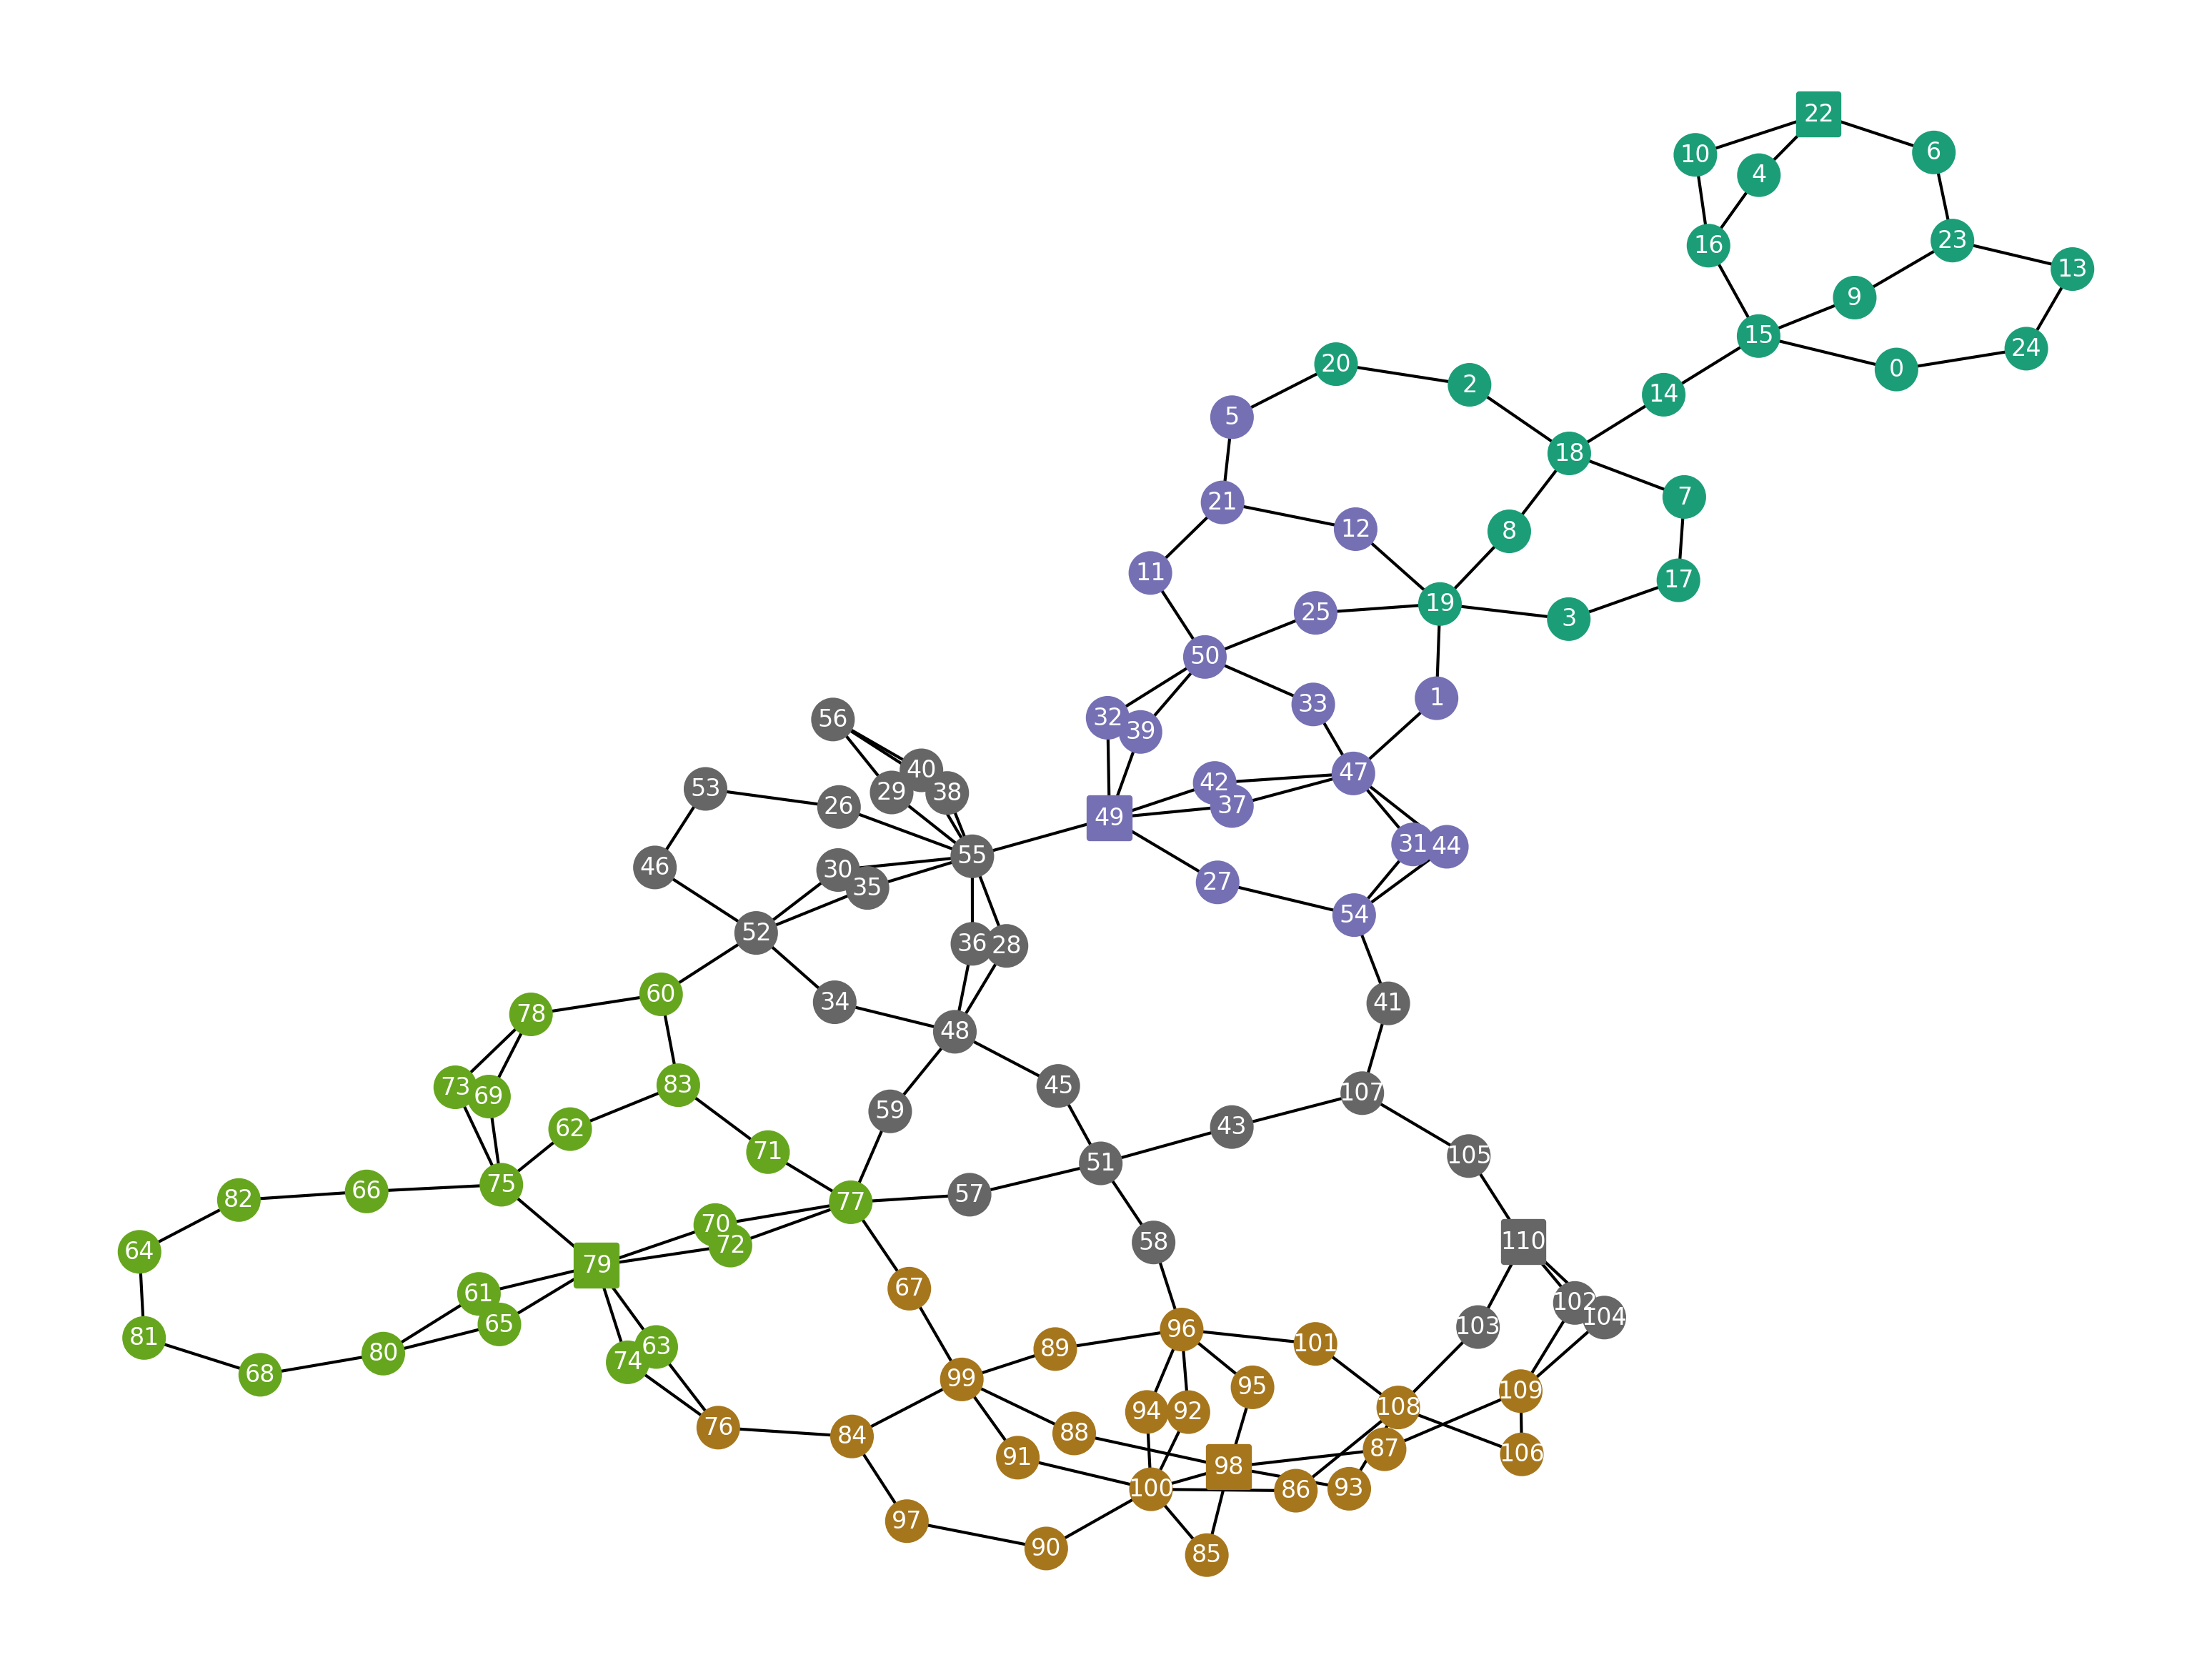
\includegraphics[width=\linewidth]{img/switchstate_exploring/swiss_suburb/topology_worst.png}
      \caption{}
      \label{fig:result:suburban:worst}
    \end{subfigure}%
    \begin{subfigure}{.5\textwidth}
      \centering
      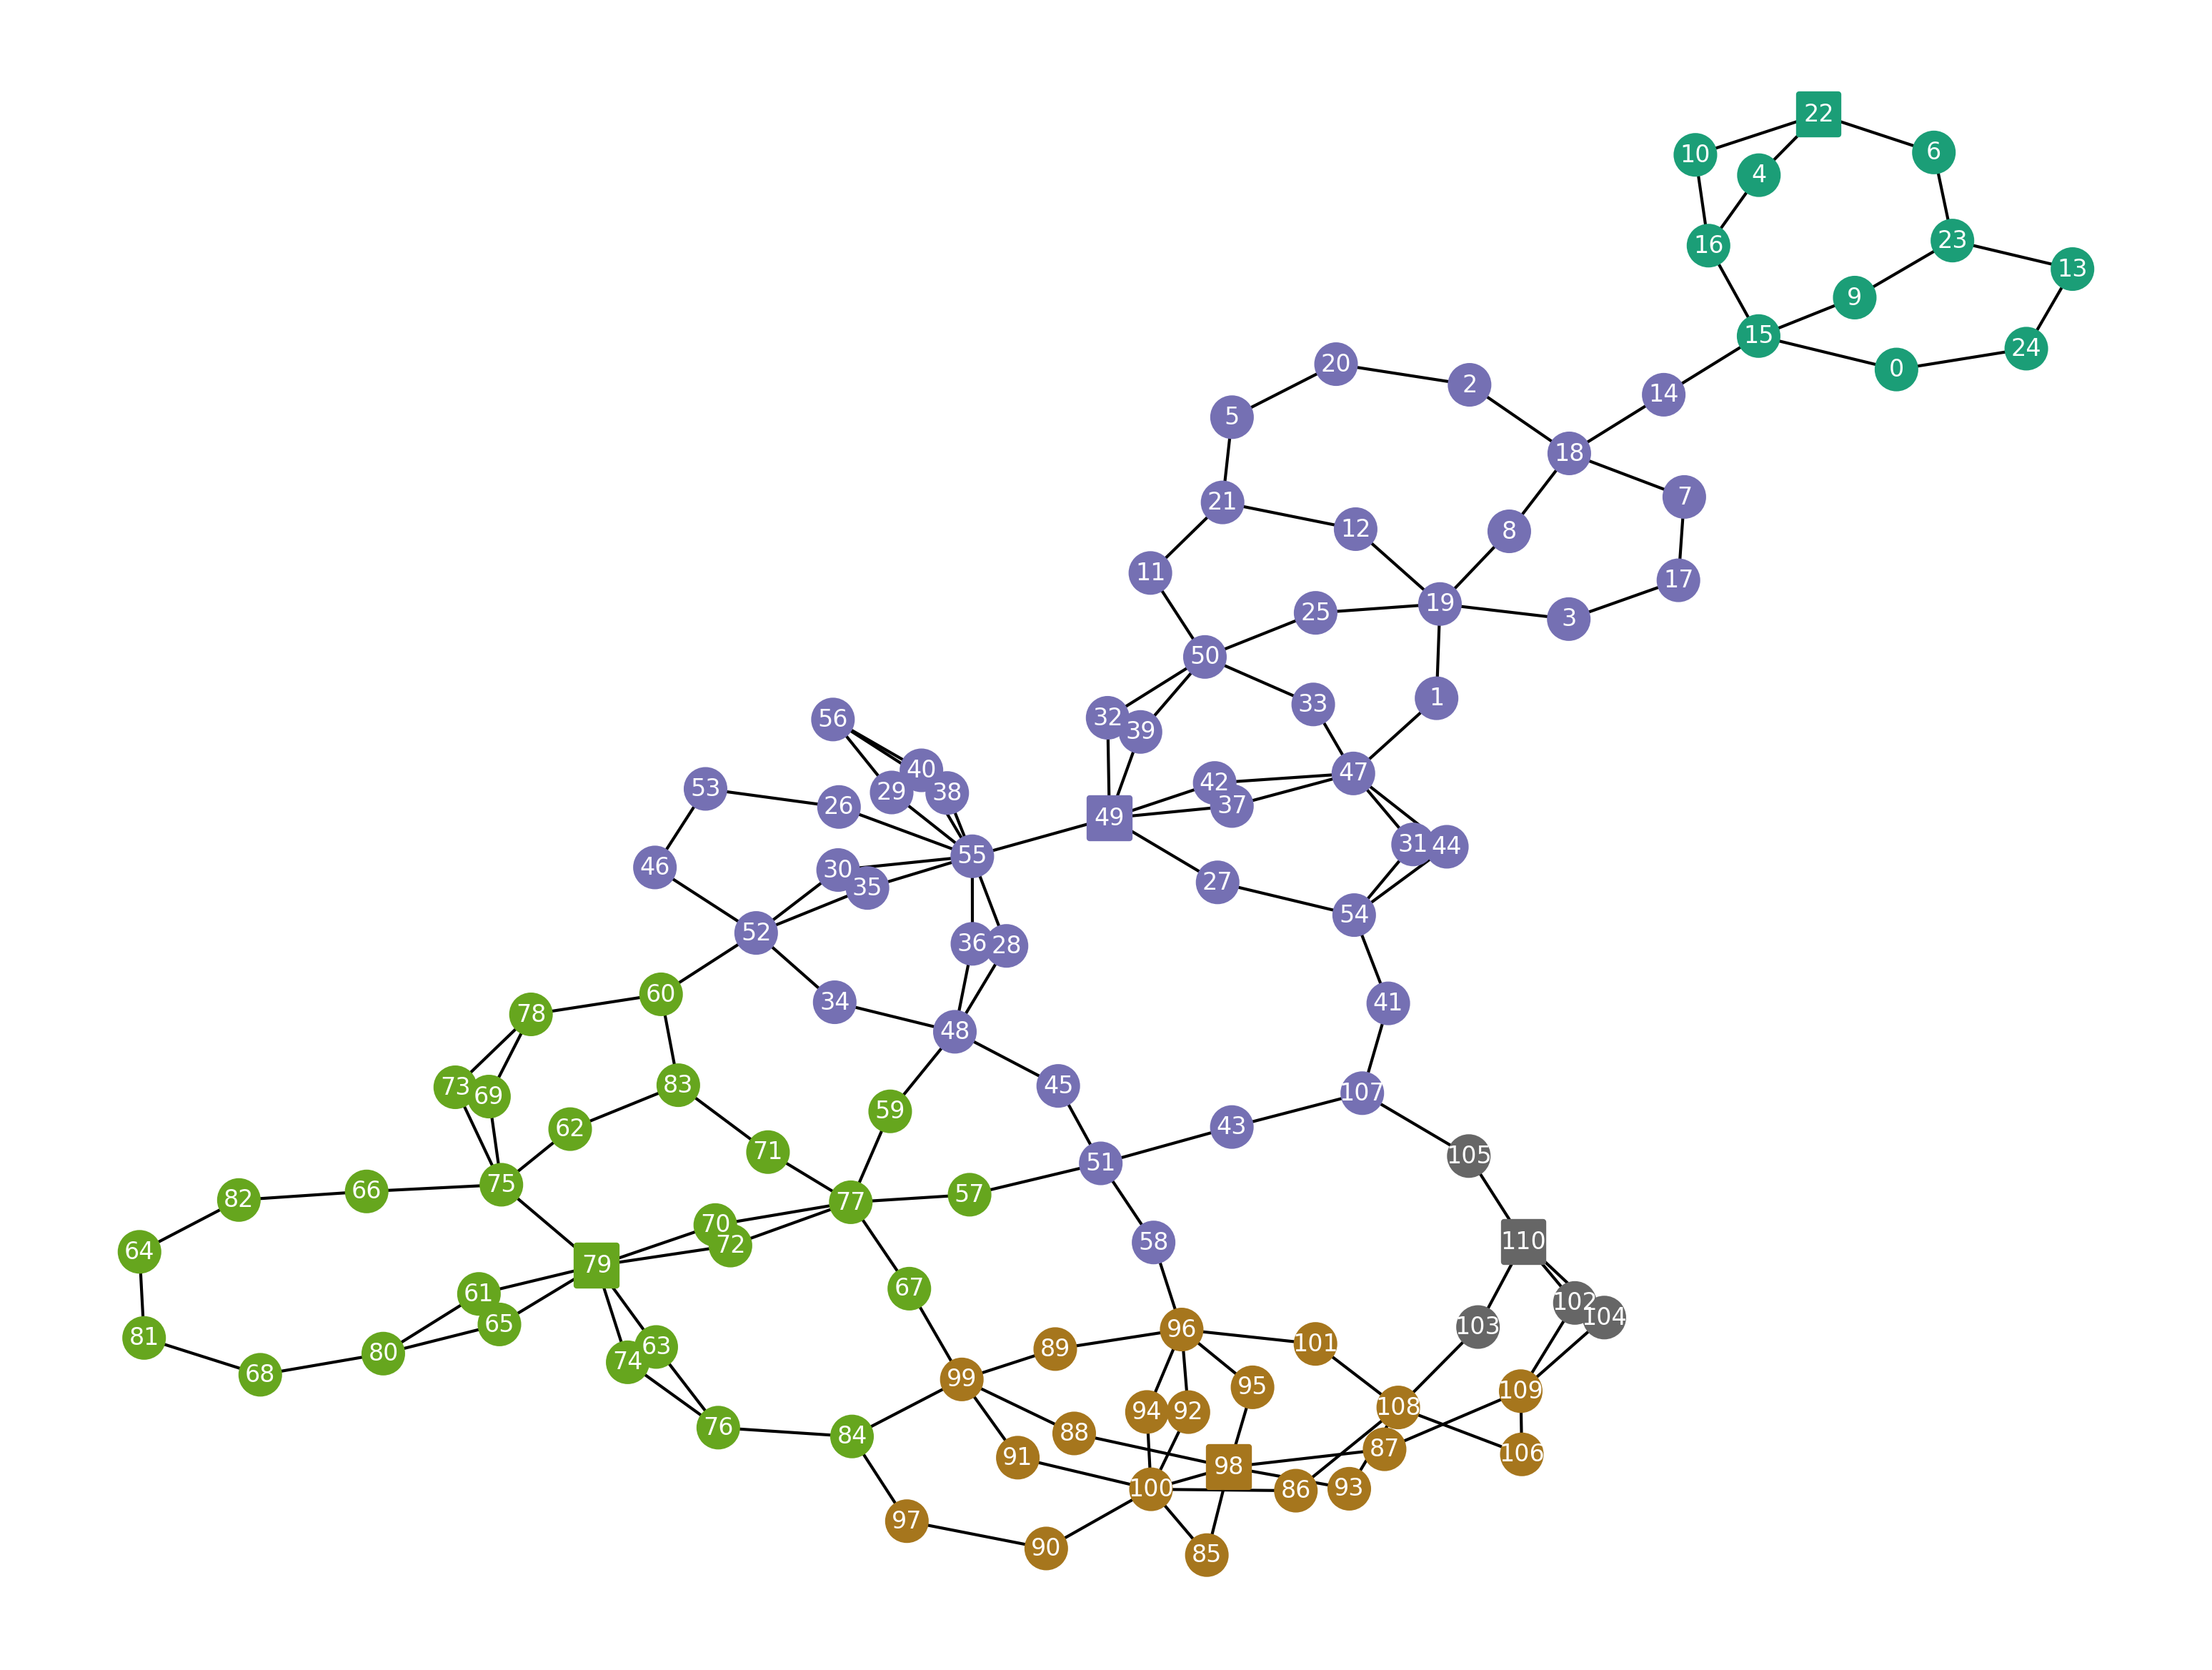
\includegraphics[width=\linewidth]{img/switchstate_exploring/swiss_suburb/topology_best.png}
      \caption{}
      \label{fig:result:suburban:best}
    \end{subfigure}
  \caption{
    Worst (a) and best (b) switch state found through random switch
    state generation in swiss suburban grid area. 
    Non-geographical layout using
    Kamada-Kawai algorithm\autocite{kamada_kawai}.
  }

This example grid area seems to present a particularly good case
for switch state improvements. \autoref{sec:appendix:urban2} contains
switch state data for the "Urban 2" grid area. Whilst improvements
to various operational parameters can be seen there as well, the improvements
are not as large. From the limited testing over grid areas that we 
have conducted, the potential for switch state improvements seems to be
bigger in suburban areas rather than in urban ones. This conclusion is
supported by the switch state data on the "Suburb 2" grid area
which can be found in \autoref{sec:appendix:suburb2}.\\
A hypothesis is that suburban areas have more renewables and thus more
generation at the local level. This could open up the possibility
for local supply where electricity comes from neighbouring households in
these areas, which the improved switch states unlock.\\
However, other factors could also be at play here. A more thorough investigation
across more grid areas is needed.

\end{figure}
